\chapter{Discussion and Conclusion}
\label{ch:conclusion}

\begin{figure}[ht]
	\centering
	\begin{subfigure}[t]{0.5\textwidth}
		\centering
		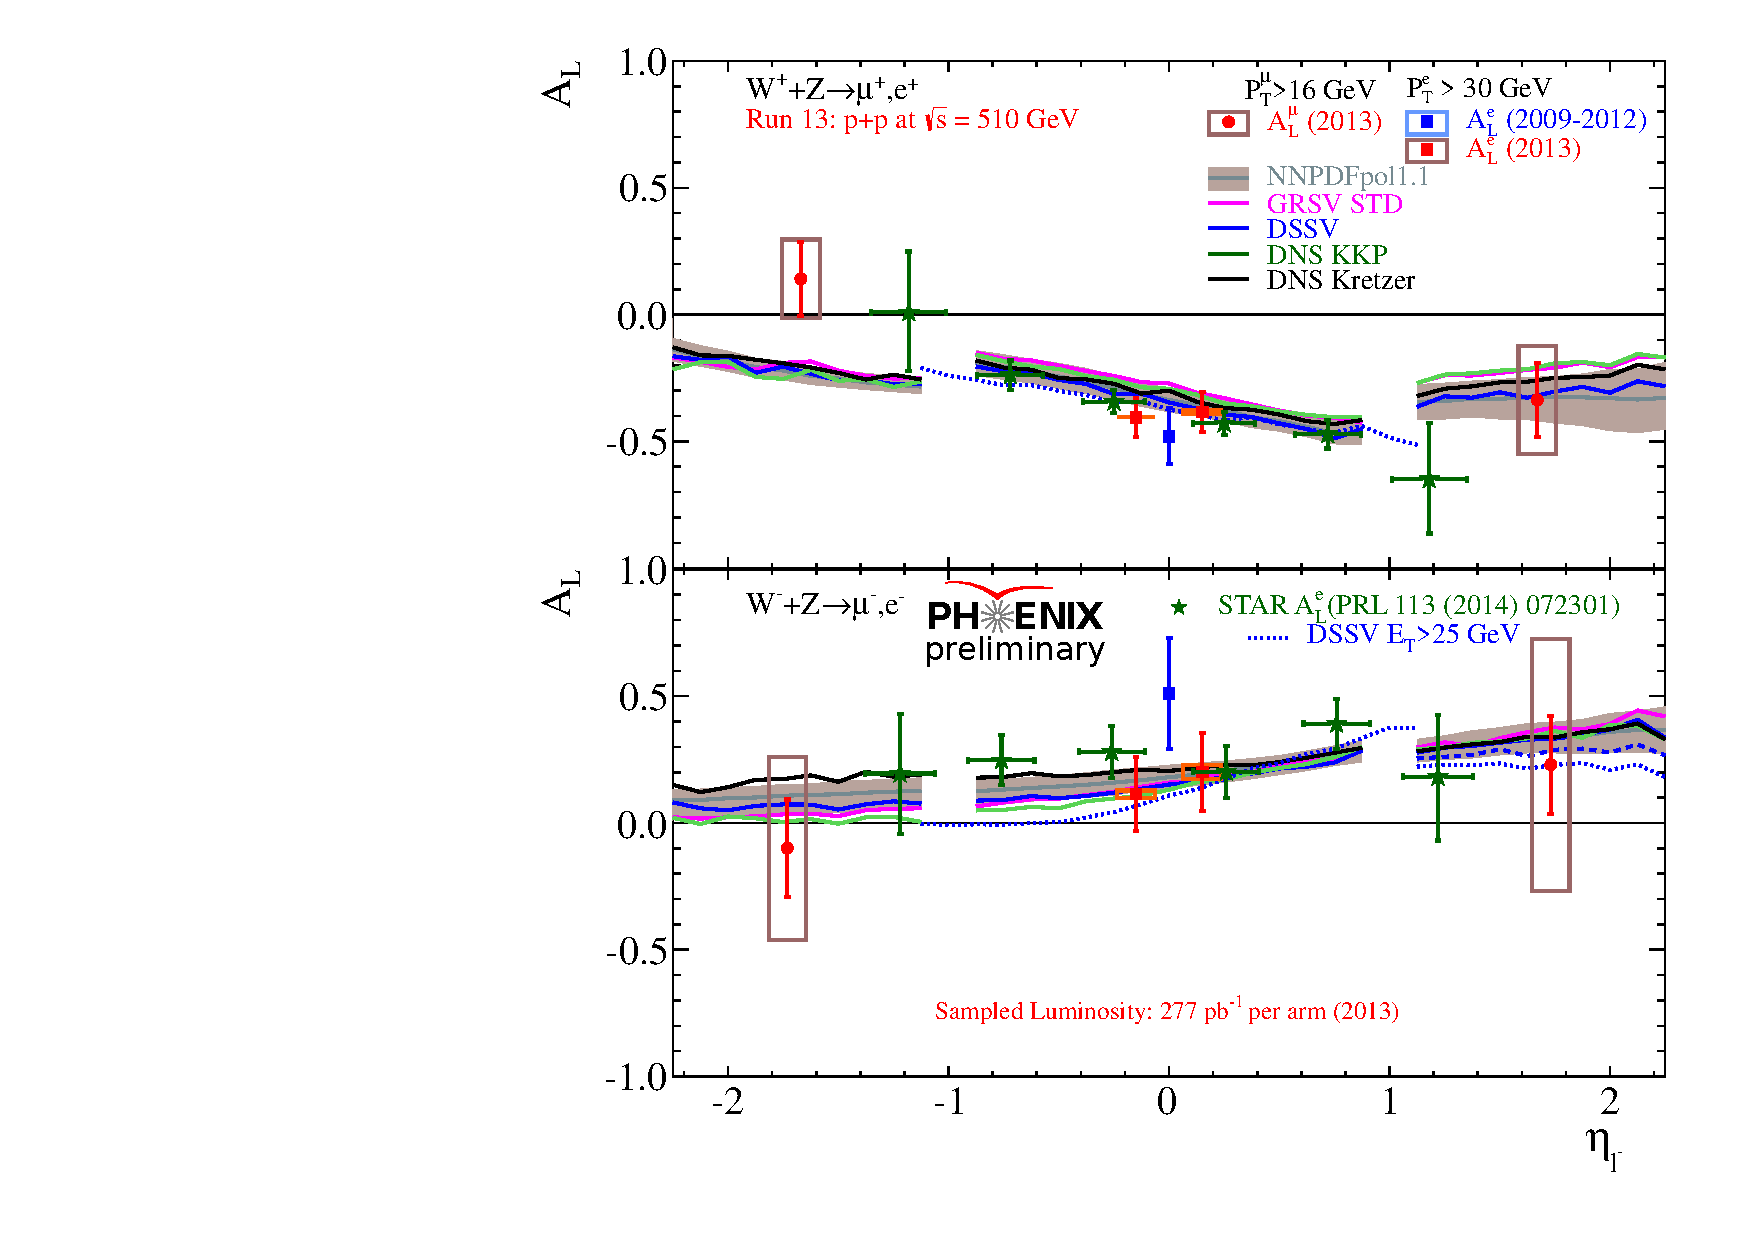
\includegraphics[width=0.95\linewidth]{./figures/prelim_AL_2bins.pdf}
	\end{subfigure}%
	\begin{subfigure}[t]{0.5\textwidth}
		\centering
		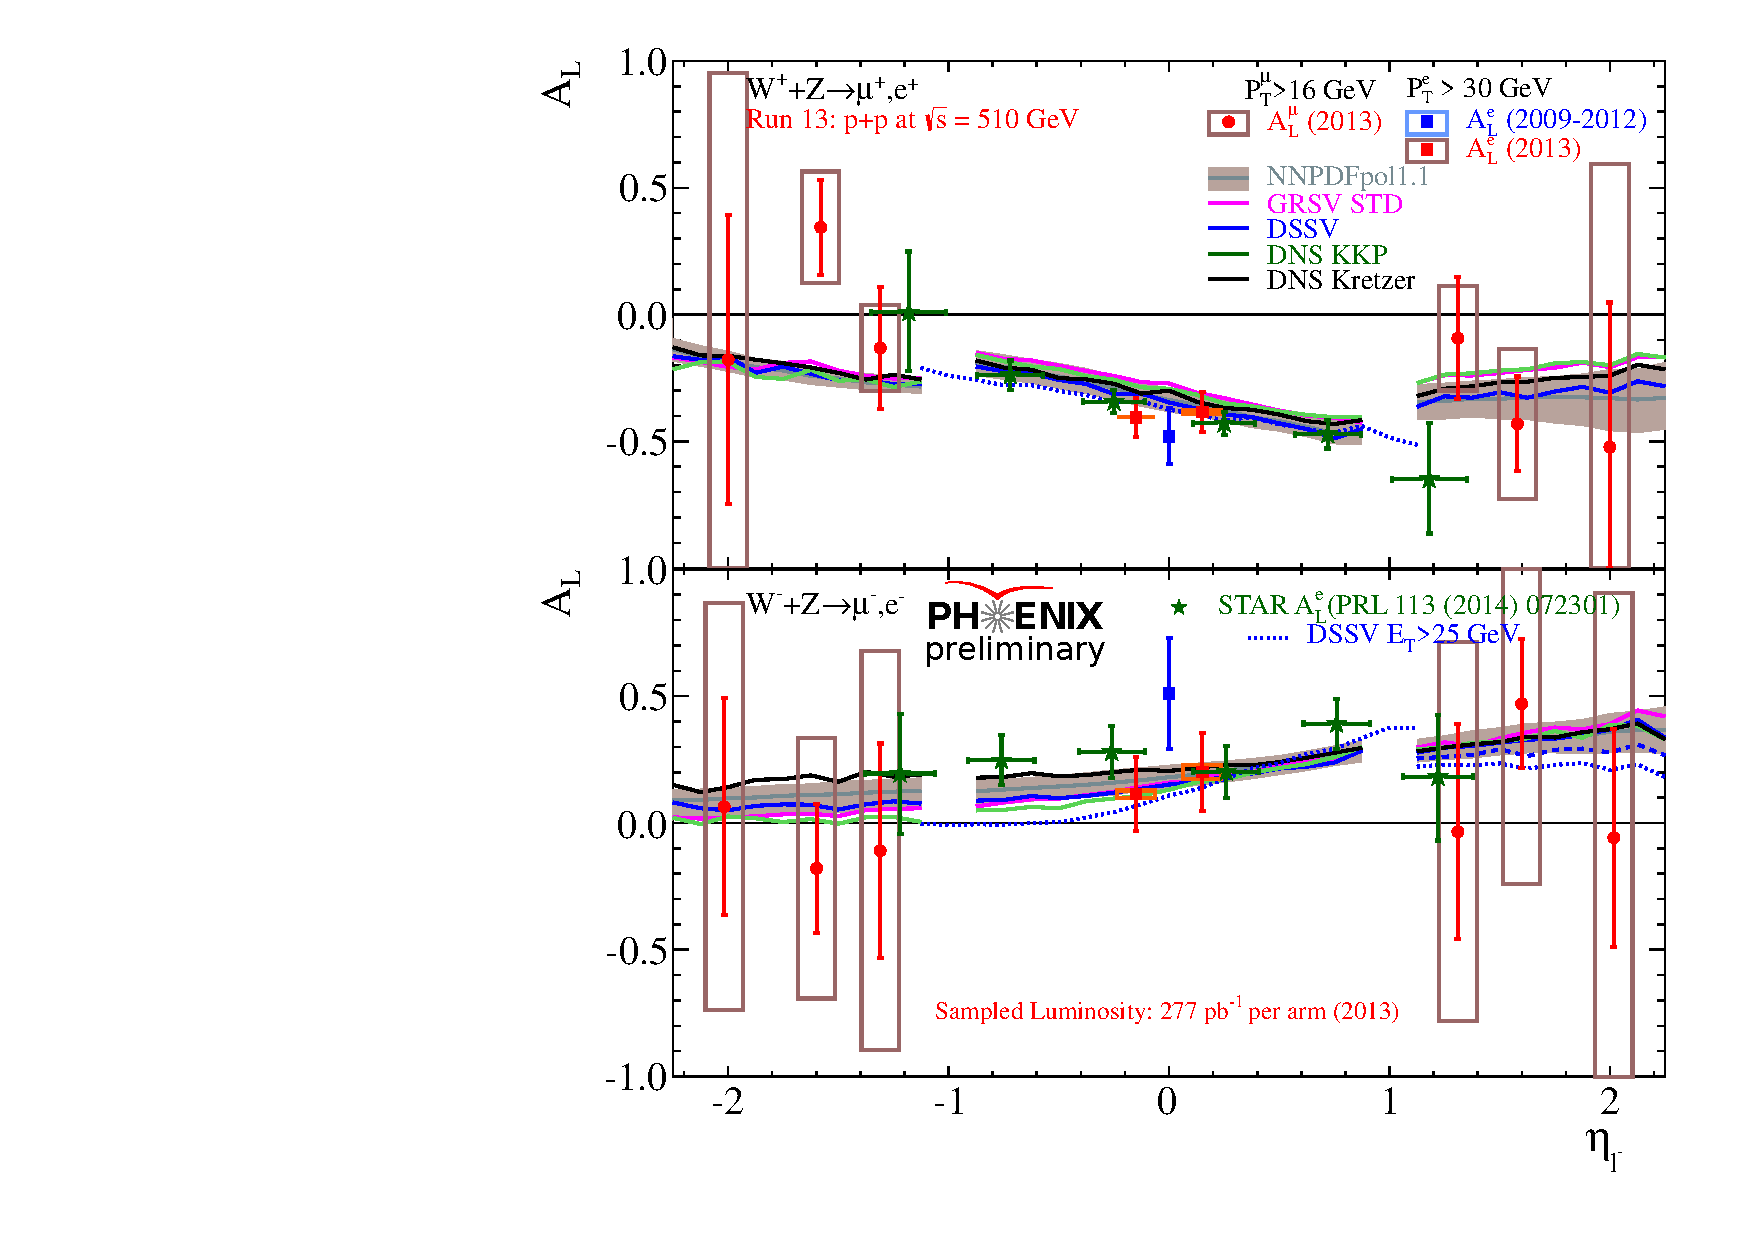
\includegraphics[width=0.95\linewidth]{./figures/prelim_AL_6bins.pdf}
	\end{subfigure}
	\caption{
		Preliminary asymmetries from Run 13, reproduced from
		Figure~\ref{fig:al_preliminary_three_eta} and
		Figure~\ref{fig:al_preliminary_standard}
	}
	\label{fig:asymmetries_preliminary}
\end{figure}

The PHENIX results on the Asymmetry (Figure~\ref{fig:asymmetries_preliminary})
put an important constraint on the polarized parton distribution functions and
therefore the spin contributions of the sea-quarks to the total proton spin. Due
to the kinematic mixing between the quark flavors ($\Delta\bar{u},
\Delta\bar{d}, u, d$) perfect separation of the quark helicities cannot be
achieved. However, as seen in Figure~\ref{fig:asymmetries_preliminary}, our
measurement (red boxed data points) overlaps the regions of largest uncertainty
in the projections in the asymmetries. These regions of large asymmetry are the
dominated by uncertainties in the anti-quark polarization. In the forward
kinematic region, the asymmetries for the $W-$ give enhanced sensitivity to
sea-quark polarization whereas the $W+$ contains mixed contributions.
Therefore, moving forward, we expect the NNPDF global fits to the world data set
to be improved with the addition of our data. This gives us a clearer picture of
the spin contribution of the anti-quarks to the total proton spin, but we still
need more data to finalize its contribution.

The future of this analysis in particular depends crucially on our understanding
of the signal to background ratio. The results from unbinned maximum likelihood
fit, discussed in Section~\ref{sec:sbr}, are the principal source of uncertainty
in this analysis. In particular, it is difficult to estimate the probability
distribution functions associated with the hadronic background. By improving our
understanding of this process, the uncertainty of the extended unbinned
maximum likelihood fit would be reduced, leading to reduced uncertainties in the
measured asymmetries. The only way to reduce the uncertainty associated with the
hadronic processes would be to use finely tuned simulations with trillions of
simulated events. This in turn would require a deep understanding of the
relatively rare hadronic background processes.

Barring the computational difficulty of obtaining a realistic simulation of the
hadronic background processes, producing such simulations may not fully solve the
challenge of differentiating signal from background. It may be that the
probability distribution functions associated with the hadronic background look
too similar to those associated with the signal process. In this case, our model
would have difficulty discerning signal and background events.

Further investigation into obtaining better models for the hadronic background,
or potentially better approaches for extracting the hadronic background
distributions directly from the data set are two potential strategies for
improving this analysis by reducing the associated uncertainty from the signal to
background ratio fits. Other strategies might involve further upgrades to the
detectors to enable better tracking, or more shielding to reduce punch through
hadrons.

Looking forward to the future measurements to help constrain the spin structure
of the proton - the frontier of future measurements lie with the construction of
an electron-ion collider~\cite{Aschenauer2016}. Even with the completion of the
RHIC $W$ physics program, some elements of the light proton sea polarization are
known with little precision - for example - $\Delta\bar{d}-\Delta\bar{u}$.
Strange quarks may also contribute to proton spin in some way, and this
contribution is not well understood. More than anything else, the Electron-Ion
collider will allow for the precise study of the polarized proton structure
function, $g_1(x,Q^2)$ and its scaling violation over a broad range of $x$.
Especially at scales $x < 0.004$ and $Q^2 > 1 GeV^2$, $g1$ is totally
unexplored~\cite{Accardi2012}. Finally, although the longitudinal spin structure
is explored in this thesis, the transverse spin structure must be studied to
obtain a full understanding of the three dimensional spin structure of the
proton.
